\section{LOPA analízis}
A LOPA vizsgálat során a következő forgatókönyvet fogom elemezni: A kerékcsúszás prevenciós modul túl sokáig (> 3 sec) tartja fékezetlen állapotban a rendszert miközben fékezési parancs van kiadva.

HAZOP tanulmány során derült fény erre a potenciális hibára. 
A tanulmány alapján kijelenthető, hogy a eset kiváltó hiba potenciálisan a kerékcsúszás prevenciós alrendszer beragadása egy olyan állapotba, ahol jelentősen csökkentett fékerő kerül kivezérlésre a végős beavatkozóhoz.

Ez különböző módokon lehetséges, amiknek további elemzése nem célja a vizsgálatnak, de lehet processzor, memória esetleg a vezérlést végrehajtó hardver hibája.
Továbbá tudjuk, hogy ez a hiba $4\times10^{-4} {1/h}$ frekvenciával fordul elő.

A lehetséges következmények között feltárva lett, olyan kimenetel is, hogy a hiba akár halálesethez is vezethet.
Ezért a \ref{tab:serverity} táblázat alapján a hiba \emph{Kritikus} besorolást kap.
A megadott hibarátát figyelembe véve a \ref{tab:freqency} táblázat szerint az előfordulás besorolása \emph{Alkalmi} kategóriájú.

A fentiek alapján a következő megállapítás fogalmazhatódhat meg az hibamód elfogadhatóságáról: A kapott besorolások alapján bármilyen enyhítő körülmény nélkül a kockázat elfogadási mátrix (lásd: \ref{tab:risk_mat}. táblázat) alapján \emph{Nem kívánatos} besorolást kap.
Ez csak akkor elfogadható, ha azt lehetséges tovább csökkenteni.

\subsection{Független Védelmi Rétegek vizsgálata}
Ahhoz, hogy eszközt, rendszert vagy funkciót független védelmi rétegnek (továbbiakban IPL\footnote{Independent Protection Layer}) lehessen tekinteni a következőnek kell teljesülni\cite{LOPABOOK}:
\begin{itemize}
    \item \emph{hatékonyan} megakadályozza következményt ha úgy működik, ahogy tervezték
    \item \emph{független} a kezdő/kiváltó eseménytől és a többi IPL összes komponensétől, ami szerepel a forgatókönyvben
    \item \emph{auditálható}, az elvárt viselkedés valamilyen módon validálható/bizonyítható
\end{itemize}

Az IPL-eknek két altípusát különböztetjük meg: (1) Passzív IPL, (2) Aktív IPL.

A passzív IPL-eknek nem szükséges, hogy beavatkozzanak a folyamatba ők eredendően csökkentik a kockázatot.
Az irodalomban számtalan példa található a kémiai iparágban használható passzív védelmi mechanizmusokról, de a jelen problémához nem alkalmazható ilyen elven működő eszköz.

Az aktív IPL-ek valamilyen érzékelő segítségével képes egyik állapotból a másikba kerülni ezáltal megváltoztatva a folyamatot.
Ezek egy lehetséges felépítését a \ref{fig:activeIPL}. ábra szemlélteti.
\begin{figure}
    \footnotesize
    \centering
    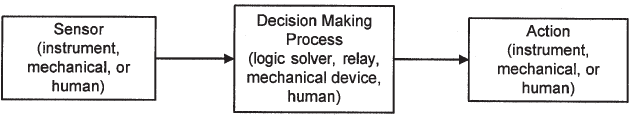
\includegraphics[width=100mm, keepaspectratio]{figures/lopa_active_IPL.png}
    \caption{Egy aktív IPL felépítése. Forrás: \cite{LOPABOOK}}
    \label{fig:activeIPL}
\end{figure}

A rendszer jelenlegi tervében sajnos nem szerepel ilyen elem. 
De szerencsére az iparágban található erre a problémakörbe megfelelő modul, amit fel lehet használni a probléma kiküszöbölésére.
Ez pedig a megfigyelő (watchdog) funkcionalitás, mely monitorozza a WSP\footnote{WheelSlide Protection} működését.

Az IPL-ek hatékonyságát az eléréskori hiba valószínűsége (PFD\footnote{Probability of Failure on Demand}) határozza meg.

\subsection{Frekvencia számítás}
Az esemény következményének frekvenciáját az alábbi egyenlettel lehet megadni:
\begin{equation}
    f^C = f^I\times\prod^{J}_{j=1}{{PFD}_j}
\end{equation}
\label{eq:lopa}
Ahol,

$f^C$ a kimenetel frekvenciája

$f^I$ a kezdeményező esemény frekvenciája és

$PDF_j$ a j-edik IPL hibájának valószínűsége, ami védelmet nyújt a kimenetellel szemben.

Néhányaknak szemetszúhatott már, hogy az IPL-ek esetében On-Demand hiba valószínűségről beszél a szakirodalom, míg a vasútiparban általában folytonos módban vannak megadva a tűrésértékek.
Ezért fontos kiemelni, hogy konverzió nélkül nem alkalmazható a fenti egyenlet.

A két szabványrendszer kapcsolatát a \ref{tab:sil_thr_pfd} táblázat írja le.
Mivel a rendszer tisztán elektronikus ezért a fejezet elején leírtak szerint a rendszer megbízhatósága $r(t) = e^{-\lambda t}$ közelíthető.
Továbbá szitén fentebb említettek szerint a rendszer élettartama 30 év, évi 5000 órás használattal.

Ezért annak a valószínűséget, hogy a rendszer meghibásodik az élettartama során (150 000 óra): $1-e^{-\lambda*150000}$
Ezt behelyettesítve a THR-rel megkapható az átlagos PFD értéke.

\begin{table}
    \footnotesize
    \centering
    \begin{tabular}{ |c|c|c| }
        \hline
        SIL besorolás & THR\footnote{Tolerable Hazard Rate} & PFD \\
        \hline
        SIL4 & $1e^{-8} < f \leq 1e^{-9}$ & $1e^{-3} < f \leq 1e^{-4}$ \\
        \hline
        SIL3 & $1e^{-7} < f \leq 1e^{-8}$ & $1e^{-2} < f \leq 1e^{-3}$ \\
        \hline
        SIL2 & $1e^{-6} < f \leq 1e^{-7}$ & $1e^{-1} < f \leq 1e^{-2}$ \\
        \hline
        SIL1 & $1e^{-5} < f \leq 1e^{-6}$ & $9e^{-1} < f \leq 1e^{-1}$ \\
        \hline
    \end{tabular}
    \caption{A SIL besorolások kapcsolata a THRrel és a PFDvel.}
    \label{tab:sil_thr_pfd}
\end{table}

A forgatókönyhöz tartozó tűrhető kockázat a fenti elemzésekből adodóan ${THR} > 1e^{-7}$.
A csökkentés nélküli frekvencia $1e^{-4}$, tehát a folyamat során legalább három nagyságrenddel kell csökkenteni a lehetséges előfordulást.

Ez úgy érhető el, ha a watchdog funkcióból SIF\footnote{Safety Instrumented Function}, azaz biztonság-kritikus funkció keletkezik SIL4-es besorolással, hiszen ekkor a fenti egyenlet szerint
\begin{align}
    \mathbf{f}^C&= \mathbf{f}^I\times \prod^{J}_{j=1}{\mathbf{PDF}_{j}} \\
     &= 1e^{-4}\prod 1e^{-3} \\
     &= 1e^{-7}
\end{align}
A csökkentett hibaelőfordulás már csak $f > 1e^{-7}$, ami tolerálható.

Ezért a vizsgálat utáni javaslat, hogy a folyamatot fel kell instrumentálni egy hibadetektáló alrendszerrel.
Továbbá, mivel egy SIL4-es funkció kifejlesztése nagyon költséges a vállaltra nézve és feltételezve, hogy a SIL2-es funkció ténylegesen képes két nagyságrendű csökkentésre lehetséges még egy modifikációs javaslat.
Néhány helyzetben költséghatékonyabb kifejleszteni két SIL2-es funkciót/terméket mint egy SIL4-est.
Ezek alapján a másik javaslat, hogy WSP funkcióból is képeznek egy SIF-et, amely így képes csökkenteni saját hibáit ezáltal az alap frekvenciát is.
Ha mind a WPS, mind a WPS watchdog részegységek SIL2-es besorolással rendelkeznek az eredő csökkentés $1e^{-4}$, amivel teljesíthető a tűrhető hibaráta követelménye.